\documentclass[czech,bachelor]{diploma}

\usepackage[autostyle=true,czech=quotes]{csquotes}
\usepackage[backend=biber, style=iso-numeric, alldates=iso]{biblatex}
\usepackage{dcolumn}
\usepackage{subfig}
\usepackage[cpp]{diplomalst}

\addbibresource{biblatex.bib}

\ThesisAuthor{Ratmir Gaitov}
\ThesisSupervisor{Ing. Petr Olivka, Ph.D.}
\CzechThesisTitle{Autonomní řízení auto - optimalizace řízení dle pohybových senzorů}
\EnglishThesisTitle{Autonomous Car Control - Speed Optimization According to Motion Sensors}
\SubmissionYear{2024}
\ThesisAssignmentFileName{ThesisAssignment.pdf}

\Acknowledgement{Rád bych na tomto místě poděkoval mého vědoucího Petra Olivku, který mi s prací pomohl, protože bez nich by tato práce nevznikla.}

\CzechAbstract{
Tato práce popisuje ovládání modelu automobilu používaného na mezinárodní soutěží NXP Cup, konkretně korigování rychlosti jízdy pomocí pohybových senzorů.
Jsou provedeny testy různých senzoru a signálových filtru, ze kterých pak vybraná nejlepší konfigurace.
Tyto vybrané signálové filtry pak implementovaný v kombinace se vhodnými senzory.
}
\CzechKeywords{Automatické regulování rychlosti; Signálové filtry; NXP Cup; FRDM-K66F}

\EnglishAbstract{This paper describes the control of a model car used in the international NXP Cup competition, specifically the correction of driving speed using motion sensors.
Tests of different sensor and signal filters are performed, from which the best configuration is then selected.
These selected signal filters are then implemented in combination with suitable sensors.}
\EnglishKeywords{Automatic speed control; Signal filters; NXP Cup; FRDM-K66F}

\AddAcronym{ARM}{Advanced RISC Machine}
\AddAcronym{GPIO}{General-Purpose Input/Output}
\AddAcronym{IMU}{Inertial Measurement Unit}
\AddAcronym{LED}{Light-Emitting Diode}
\AddAcronym{MCU}{Micro Controller Unit}
\AddAcronym{MEMS}{Micro-Electro-Mechanical System}
\AddAcronym{NiMH}{Nickel-Metal Hydride}
\AddAcronym{PWM}{Pulse Width Modulation}
\AddAcronym{RAM}{Random Access Memory}
\AddAcronym{SDHC}{Secure Digital High Capacity}
\AddAcronym{WiFi}{Wireless Fidelity}

\newcolumntype{d}[1]{D{,}{,}{#1}}

\begin{document}
\MakeTitlePages

\listoffigures
\clearpage

\listoftables
\clearpage

\chapter*{Úvod}
\label{sec:Introduction}
\addcontentsline{toc}{chapter}{\protect\numberline{}Úvod}\

Autonomní řízení automobilů je v~současné době velmi populárním tématem, přičemž
výrobci automobilů se předhánějí o~prvenství v~této oblasti. Jedná se především
o~velmi komplexní oblast, kde musí být správně vyřešeny všechny možné situace, jelikož
jakýkoliv přehlédnutý detail může způsobit újmu na zdraví. Z~tohoto důvodu je
autonomní řízení částí populace stále vnímáno jako něco  nepřijatelného, ovšem
zvyšující se rychlost vývoje naznačuje, že v~následujících letech dojde k~významnému
pokroku v~této oblasti a~setkávání autonomně řízenými auty bude běžným jevem.

V~této bakalářské práci bude popsán způsob automatického řízení auta a~korekce 
rychlosti na základě informací z~pohybových senzorů. Práce začne popisem modelu 
automobilu pro testování. Následně budou popsány algoritmy pro automatické a~manuální 
řízení. Další část se bude zabývat metodami pro zobrazování a~ukládání hodnot dat auta 
během jízdy. Poté budou otestovány a~vybrány vhodné senzory a~filtry pro detekci fáze 
jízdy. V~závěrečné části práce bude popsán algoritmus pro optimalizaci rychlosti 
a~provedeno porovnání s~manuálním řízením.

\endinput
\chapter{Model automobilu}
\label{sec:CarModel}\

V~této kapitole je popsán model automobilu a~jeho jednotlivé součásti.

Model automobilu je založen na podvozku typu Alamak, která má \textbf{1 servomotor}
pro řízení a~\textbf{2 motory} pro pohon. \textbf{Podvozek Alamak} je řízen pomocí 
\textbf{NXP Freedom K66F} spolu s~modulem \textbf{POLI-TFC} 
přípojeným do GPIO pinů MCU. Detailní popis MCU a~modulu jsou v~podkapitolách 
\ref{sec:FRDM-K66F} a~\ref{sec:POLI-TFC}.

Pro manuální řízení je zapojen přijímač RC signálu \textbf{Minima 6S} do pinu
POLI-TFC shieldu. Přijímač pak přijímá signály z~vysílače \textbf{Hitec OPTIC 6 
SPORT}.

Pro komunikaci s~podvozkem Alamak je použit \textbf{WiFi Access Point}, který je
připojen k~MCU pomocí Ethernet portu. \textbf{Řádková kamera}, která je umístěna
v~přední části, se používá pro získání obrazu dráhy. Všechny součástky
jsou napájeny baterií typu \textbf{NiMH} o~napětí 7,2 V.

Celý model je zobrazen na obrázku \ref{fig:car}.
\begin{figure}[!h]
    \centering
    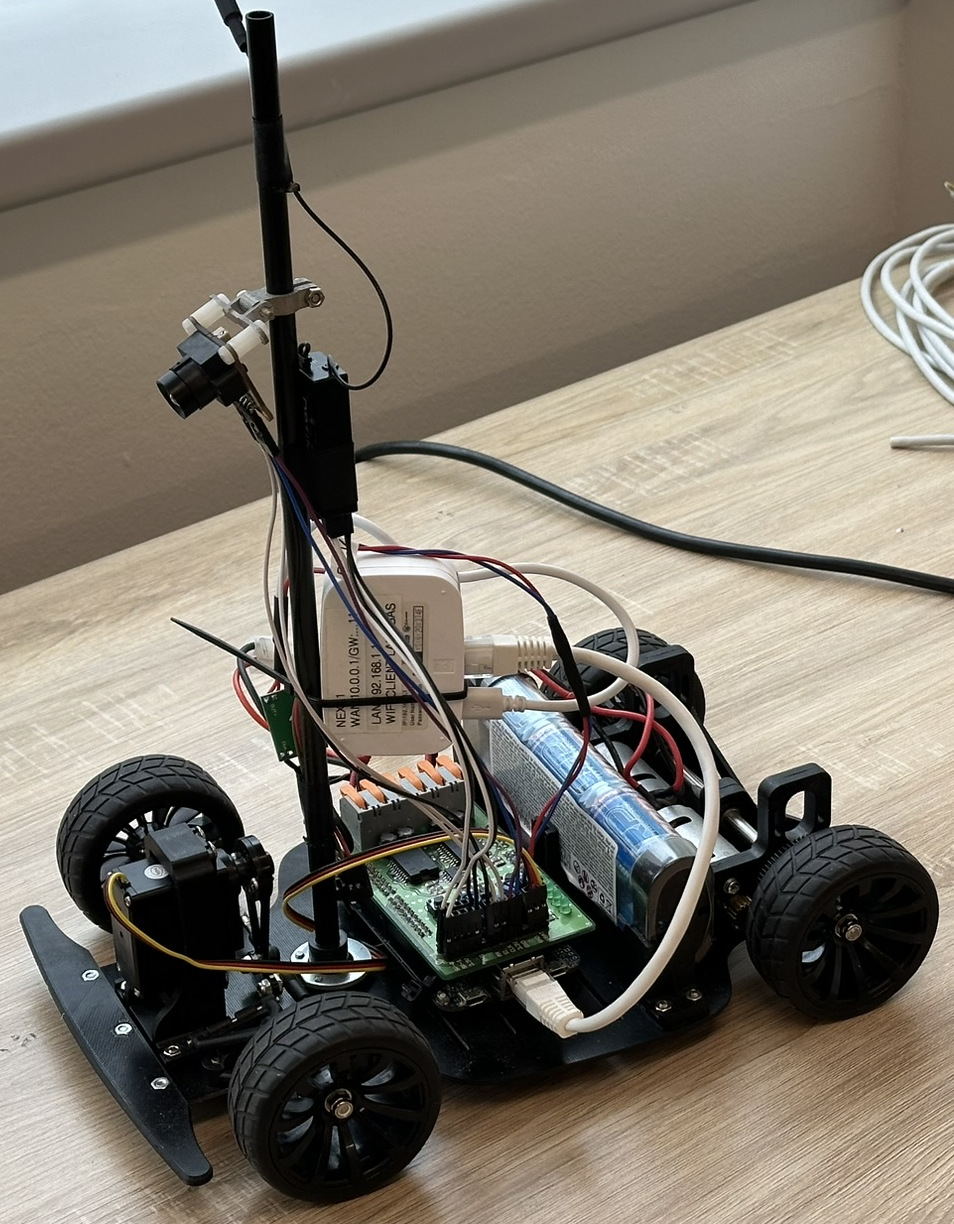
\includegraphics[width = .4\linewidth]{Figures/Car.jpeg}
    \caption{Model auta.}
    \label{fig:car}
\end{figure}

\section{FRDM-K66F}
\label{sec:FRDM-K66F}\

\textbf{FRDM-K66F} je vývojová platforma od společnosti NXP určená pro MCU řady 
Kinetis K66 a~K26. Platforma je založena na jádře \textbf{ARM© Cortex®-M4}
a~využívá model \textbf{MK66FN2M0VMD18} s~frekvencí 180 MHz, 2 MB flash paměti
a~256 KB RAM \cite{frdmk66UserGuide}.

Konektivitu zajišťují 2 micro-B USB porty, 1 ethernetový port a~54 GPIO pinů.
GPIO~piny jsou kompatibilní s~\textbf{Arduino™ R3}, čímž je poskytnuta široká škála
možností pro rozšiřující desky. Deska umožňuje bezdrátové možností konektivity
pomocí modulů Bluetooth a~RF \cite{frdmk66UserGuide}.

Pro ladění je na platformě přítomno rozhraní \textbf{OpenSDAv2.1}, které podporuje
J-Link. J-Link~je sériový programovací adaptér, který umožňuje programování
a~debugování mikrokontrolérů \cite{frdmk66UserGuide}.

Další užitečné periferie na desce zahrnují trojbarevnou LED, SDHC a~digitální MEMS
mikrofon~\cite{frdmk66UserGuide}.

Jako \textbf{inerciální měřicí jednotku} (IMU) platforma využívá akcelerometr
společně s~magnetometrem a~gyroskopem \cite{frdmk66UserGuide}.

Vývojová platforma je znázorněna na obrázku \ref{fig:FRDM-K66F}.

\section{POLI-TFC}
\label{sec:POLI-TFC}\

\textbf{POLI-TFC shield} je rozšiřující deska pro FRDM-K66F, která rozšiřuje
rozhraní pro připojení periferií k~vývojové desce. Shield obsahuje 2 konektory
pro motory, 2 servomotory, 2 rozhraní pro~připojení řádkových kamer, 2 
potenciometry, 4 DIP přepínače a~4 LED diody. 

Shield~je zobrazen na obrázku \ref{fig:POLI-TFC}.

\begin{figure}[h]
    \begin{subfigure}{0.45\textwidth}
        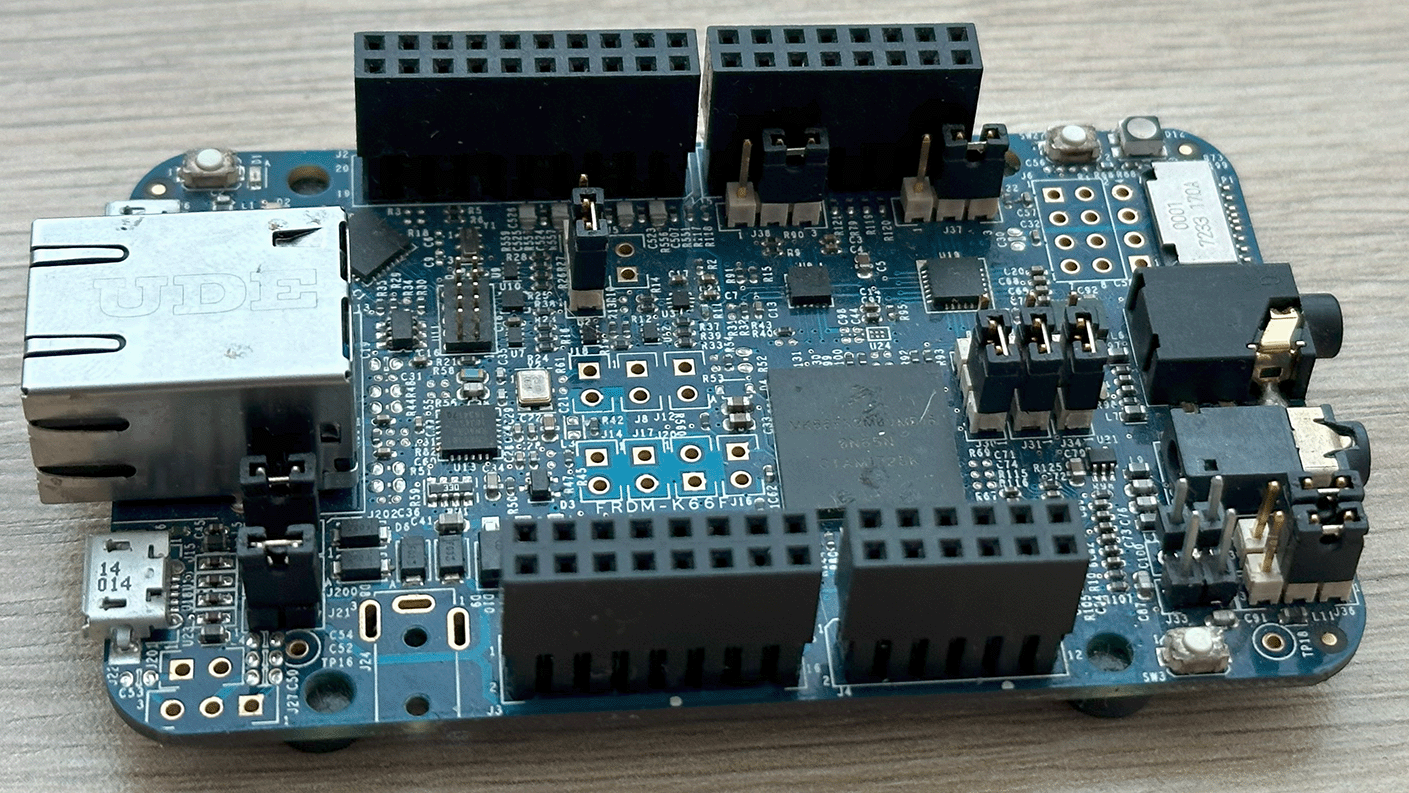
\includegraphics[width=\textwidth, height = 5cm]{Figures/FRDM-K66F.png} 
        \caption{FRDM-K66F.}
        \label{fig:FRDM-K66F}
    \end{subfigure}
    \hfill
    \begin{subfigure}{0.45\textwidth}
    	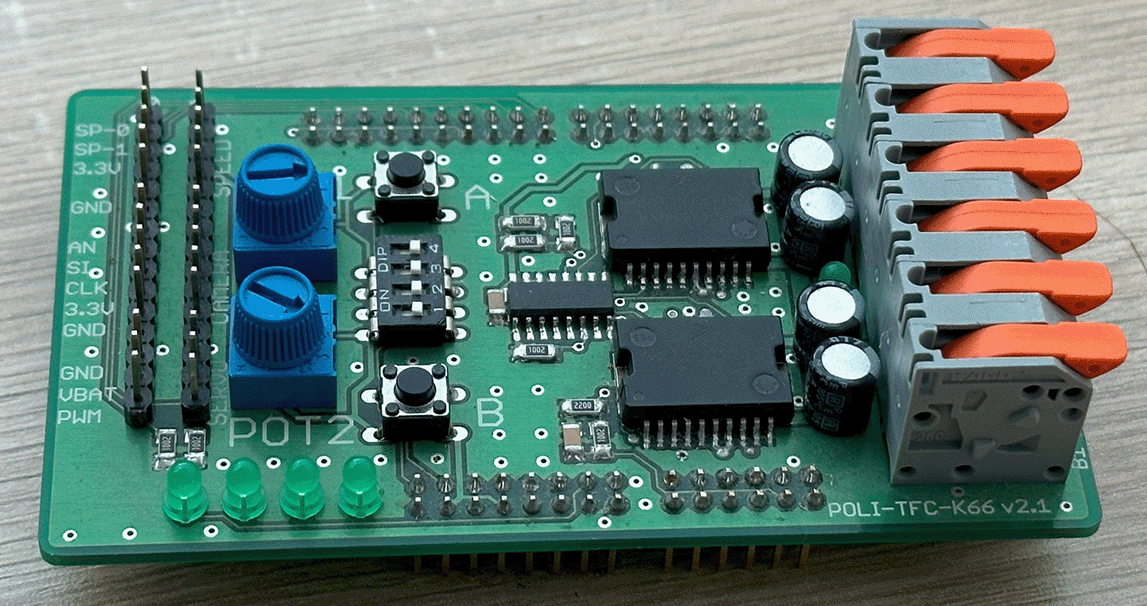
\includegraphics[width=\textwidth, height = 5cm]{Figures/POLI-TFC.png}
    	\caption{POLI-TFC.}
    	\label{fig:POLI-TFC}
	\end{subfigure}
    \caption{Vývojová platforma FRDM-K66F a~POLI-TFC shield.}
\end{figure}

\endinput
\chapter{Současný stav řešené problematiky}
\label{sec:Theory}\

V této kapitole bude popsán stav problematiky automatického řízení a pohybových
senzorů. Konkretně bude popsaná práce \uv{Krokoměr s mikropočítačem ARM}\cite{krokomer} Šigurda Filipa, který používá ve své práce akcelerometry. Následné
budou popsaný práci \uv{Autonomní řízení auta - optimalizace detekce dráhy}\cite{draha} i \uv{Mechanizmy řízení robotického auta NXP (FREESCALE)}\cite{robot},
které popisuje autonomní řízení na základe řádkové kamery a senzorů. Autoři jsou
Vojtěch Ihn a Richard Zvonek.

\section{Krokoměr s mikropočítačem ARM}\

Tato práce se zabývala vývojem krokoměru s využitím desky NXP FRDM-K64F, která je
založená na jádře ARM© Cortex®-M4. Hlavním cílem práce bylo vytvoření krokoměru,
který by byl schopen detekovat a počítat kroky uživatele.

V práci byly vybírány různé MEMS akcelerometry podle několika kritérií: možnosti
integrace na plošný spoj, cenové dostupnosti, schopnosti komunikovat s
mikrokontrolérem prostřednictvím rozhraní $I^2C$ nebo SPI, přičemž byly vybírány
výhradně tříosé akcelerometry.

Akcelerometry byly následně testovány v různých prostředích a podmínkách, které
zahrnovaly chůzi po~rovině, po trávě, do a z kopce, a také chůzi do a ze schodů.

Každé měření bylo doprovázeno dvěma krokoměry:  Xiaomi Mi Band a aplikace
\uv{Pedometer} provozovanou na mobilním telefonu Nokia 6.1. Výsledky jednotlivých
akcelerometrů v~jednotlivých situacích byli velice podobné:

\begin{table}[!h]
	\centering
	\begin{tabular}{lccc}
		\toprule
		Měření s akcelerometrem      & délka chůze & Xiaomi Mi Band & Nokia 6.1 \\
		\midrule
		NXP FXOS8700CQ               & 3m 35s      & 345            & 351       \\
		NXP MMA8452Q                 & 3m 25s      & 339            & 337       \\
		Analog Devices ADXL345       & 3m 31s      & 343            & 339       \\
		STMicroelectronics LSM303DLH & 3m 30s      & 338            & 336       \\
		\bottomrule
	\end{tabular}
	\caption{Počet kroků při chůzi do kopce s krokoměrem v ruce\cite{krokomer}.}
	\label{tab:1}
\end{table}

Dále byly otestovány a porovnány různé filtry pro odstranění šumu z naměřených dat.
Použity byly filtry typu dolní propust, a to z důvodu, že normální chůze
nepřekračuje rychlost čtyř kroků za~sekundu, což znamená, že frekvence vyšší než
4~Hz byly považovány za šum. Filtrace signálu byla prováděna pomoci filtrů s
konečnou impulzní odezvou (FIR) a s nekonečnou impulzní odezvou~(IIR).

\begin{figure}[!h]
	\centering
	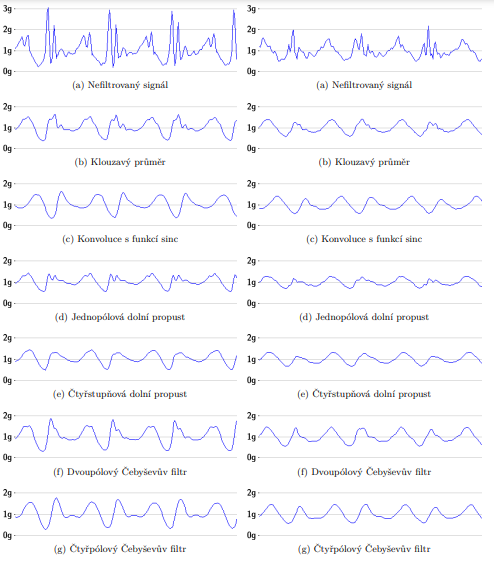
\includegraphics[width = .95\linewidth]{Figures/Filtry.png}
	\captionsetup{justification = centering}
	\caption{Čtyřsekundové ukázky aplikovaných filtrů. Vlevo: chůze po rovině s
	akcelerometrem v~kapse. Vpravo: chůze do kopce s akcelerometrem v
	kapse\cite{krokomer}.}
	\label{fig:filtr}
\end{figure}

Po porovnání filtrů byl jako nejlepší vyhodnocen dvoupólový Čebyševův filtr, který
ve srovnání s ostatními je výpočetně méně náročný a odstranil velké množství šumu se
zachováním amplitudy signálu. Výsledky aplikace filtrů jsou zobrazeny na obrázku \ref{fig:filtr}.

Pro počítání kroků byly implementovány dva způsoby detekce kroků. První z nich se
ukázal jako nevyhovující. Druhý způsob detekce kroků byl o poznáni přesnější.
Algoritmus funguje na principu stavového automatu, který má 2 stavy pro hledání
nástupních a sestupných hran.

Závěrečné testování kompletního řešení proběhlo chůzi po městě. Trasa byla přibližně
1650~metrů dlouhá. Výsledky měření byly porovnány s komerčně dostupnými krokoměry
pro ověření přesnosti navrženého řešení. Tabulka \ref{tab:2}  zobrazuje počty
naměřených kroků jednotlivými krokoměry.

Testování ukázalo, že výsledky jsou velmi podobné výsledkům ostatních dvou
krokoměrů\cite{krokomer}.

\begin{table}[!h]
	\centering
	\begin{tabular}{lcccc}
		\toprule
		Umístění krokoměru & délka chůze & Xiaomi Mi Band & Nokia 6.1 & FRDM-K64F \\
		\midrule
		V kapse            & 18m 46s     & 1986           & 2013      & 2021      \\
		V ruce             & 18m 36s     & 1993           & 2007      & 2010      \\
		\bottomrule
	\end{tabular}
	\caption{Počet kroků při závěrečném měření\cite{krokomer}.}
	\label{tab:2}
	\vspace{-10pt}
\end{table}

\section{Autonomní řízení auta - optimalizace detekce dráhy}\

Tato práce se zaměřila na zpracování obrazu získaného z řádkové kamery a na následné
vyhledávání okrajových čar dráhy s využitím různých typů objektivů a filtrů. Cílem
bylo najít optimální kombinaci, která by umožňovala nejpřesnější detekci dráhy pro
autonomní řízení vozidla. Pro dosažení tohoto cíle práce zkoumala různé metody a
techniky zpracování obrazu, včetně výběru a testování objektivů kamery, aplikaci
filtrů pro zlepšení kvality obrazu a implementaci algoritmů pro~efektivní detekci
dráhy.

Finální výběr kamery a objektivu byl založen na schopnosti kamer efektivně detekovat
okrajové čáry za různých světelných podmínek.

Dále byly otestovány různé kombinace filtrů pro redukci šumu, detekci hran a
prahování. Ve~výsledku byly pro implementaci vybrány 4 filtry: mediánový filtr,
Gaussův filtr, morfologický gradient a Otsu prahování.

Algoritmus byl testován při umělém osvětlení i při denním světle. Při rovnoměrném
umělém osvětlení byla detekce okrajových čar na dráze spolehlivá. Při denním světle
byly dosaženy slušné výsledky, které avšak nešlo považovat za ideální\cite{draha}.

\section{Mechanizmy řízení robotického auta NXP (FREESCALE)}\

V rámci této práce byl vyvinut softwarový systém pro robotický model auta. Systém
byl navržen tak, aby umožňoval autonomní navigaci po závodní dráze s využitím dat
získaných z řádkové kamery a dalších senzorů. Řídící software se skládal ze dvou
hlavních částí: zpracování obrazu z řádkové kamery a řízení na základě získaných
informací z obrazu.

Pro zpracování obrazu byly použitý: filtrování mediánem pro odstranění šumu,
normalizace obrazu pro přizpůsobení světelným podmínkám a prahování průměrem.

Pro řízení pomocí dat z kamery byl software schopen detekovat okraje dráhy a na
základě této informace řídit směr a rychlost auta. Klíčovým prvkem bylo efektivní
využití PID regulátoru.

Práce rovněž zahrnovala vývoj a integraci různých senzorů, včetně IMU a IR senzorů.
IMU~jednotka byla použita k detekci zastavení vozidla, zatímco infračervené senzory
sloužily k detekci blízkých objektů a překážek.

Následně bylo robotické auto testováno na soutěži NXP Cup, kde úspěšně zvládlo
všechny tři dodatečné disciplíny v kvalifikačním kole\cite{robot}.

\endinput


\printbibliography[title={Seznam použité literatury}]
\addcontentsline{toc}{chapter}{Seznam použité literatury}
\end{document}
